% Beginning of a chapter
% Use labels for referencing
\chapter{Context}\label{entrances} 
\section{Data description}\label{datadescription}
% this is a comment
% normal text
This section will describe the main datasource within the Synthesis Project; a PostgreSQL database containing the logs from the Wi-Fi scanners on the TU Delft campus. Each row in the wifilog table provides a data value for each column (\autoref{figure:segmentwifilog}).

\begin{figure}[H]
	\centering
	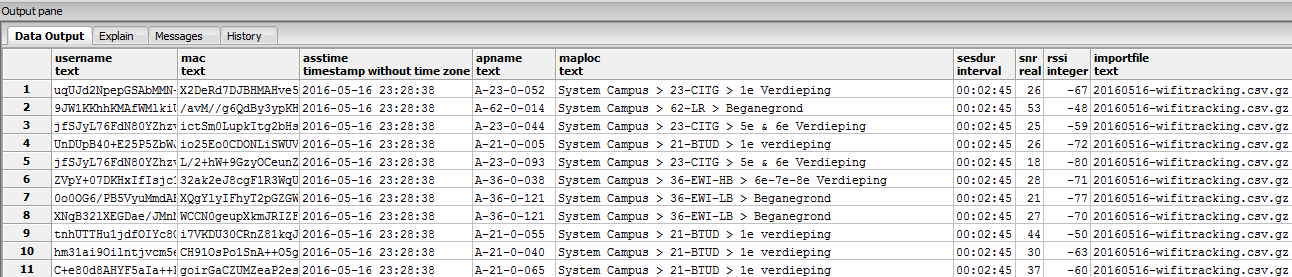
\includegraphics[scale=1]{wifilog_table.PNG}
	\captionsetup{justification=centering}
	\caption{A segment of the the main datasource; the wifilog table}
	\label{figure:segmentwifilog}
\end{figure}

The data value for each attribute (column) in the wifilog table will be described in more detail. 
\\
\textbf{username:}
The username column provides the username, as a hashed text. Every user has a unique username, but can appear in the data more than once.
\\
\textbf{mac:}
The mac column provides the media access control adress (MAC address), as a hashed text. The MAC address is a unique identifier assigned to a specific piece of hardware, such as the network adapter located in Wi-Fi devices (mobile phones, tablets, laptops etc.). So, it would be possible that a user can have more than one device connected to the Wi-Fi eduroam network.
\\
\textbf{asstime:}
The asstime is the time of which a connected device is recorded by the system.
\\
\textbf{apname:}
The apname is the name assigned to the access point. Every access point has a unique name. 
\\
\textbf{maploc:}
The maploc describes the location of the access point. There could be multiple access points with the same maploc. For instance, there are 31 access points located on the ground floor of the Faculty of Architecture.
\\
\textbf{sesdur:}
The sesdur describes the session duration of which a device is connected to the access point. Because this is not as straightforward as it seems, this will be explained more extensively.
\\
wifherwi shows the the frequency of session durations.
\\
picture
\\
The figure shows a large peak at exactly 5 minutes, a peak at approximately 5 minutes and decreasing peaks after a time interval of approximately 5 minutes. It looks like it is recording in a certain time interval in which the device is (still) connected. 
\\
In order to justify this, the query below is used to see the asstimes (and time to next asstime)
\\
\begin{lstlisting}[language=SQL]
select *, asstime_next-asstime as difference
from (
	select count(*),asstime, lead(asstime) over (order by asstime) asstime_next
	from wifilog
	where extract(day from asstime) = 4
	and extract(month from asstime) = 4
	and extract(year from asstime) = 2016
	group by asstime
	order by asstime) as subquery
\end{lstlisting}

\begin{figure}[H]
	\centering
	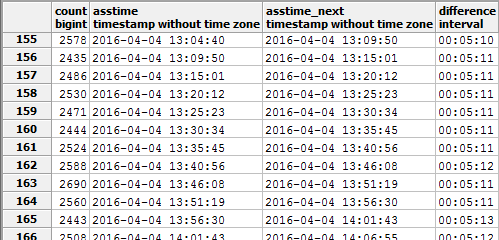
\includegraphics[scale=1]{timetonextscan.PNG}
	\captionsetup{justification=centering}
	\caption{The time and time to next scan at a random day}
	\label{figure:timetonextscan}
\end{figure}

\autoref{figure:timetonextscan} shows that the time to the next scan is 5 minutes and several seconds in all cases. Most important is to know that all access points are recording the connected device(s) is at the same time. 
\\
The way this time interval of approximately 5 minutes is in the session duration, is explained using the three depicted segments of the wifilog table.

\begin{figure}[H]
	\centering
	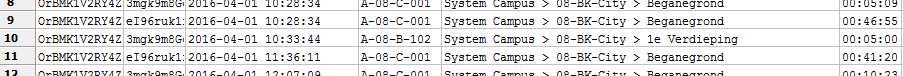
\includegraphics[scale=1]{sesdur_example1.PNG}
	\captionsetup{justification=centering}
	\caption{The device is not connected to any of the access points on the campus at the subsequent moment of recording}
	\label{sesdur_example1}
\end{figure}
The device is not connected in the subsequent moment of recording. The session duration will be exactly 5 minutes.
\\
\begin{figure}[H]
	\centering
	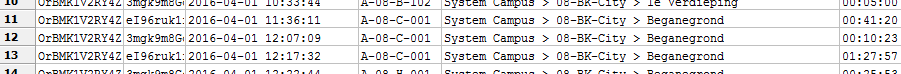
\includegraphics[scale=1]{sesdur_example2.PNG}
	\captionsetup{justification=centering}
	\caption{The device is connected to the same access point at the subsequent moment of recording}
	\label{sesdur_example2}
\end{figure}
The device is still connected to the same access point at the subsequent moment of recording. In this case the session duration will be 10 minutes and 23 seconds. This is the time interval between the first moment the device is recorded and the time the device is not recorded by the access point anymore.
\\
\begin{figure}[H]
	\centering
	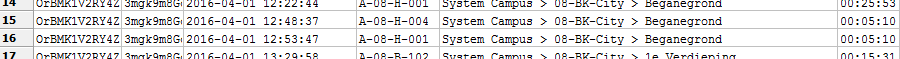
\includegraphics[scale=1]{sesdur_example3.PNG}
	\captionsetup{justification=centering}
	\caption{The device is connected to another access point at the subsequent moment of recording}
	\label{sesdur_exampl3e}
\end{figure}
Because the device is connected to an access point at the moment of recording and connected to another access point at the subsequent moment of recording, the session duration is 5 minutes and 10 seconds in this case. This is the time interval between the two moments of recording.
\\
\textbf{snr:}
The signal to noise (snr) describes a measurement that compares the signal strength to the level of background noise (in dB).
\\
\textbf{rssi:}
The received signal strength indicator (rssi) describes the received signal strength (in dB).

\section{System of APs}\label{systemofaps}
This section will describe the current layout of access points (APs) on the TU Delft campus. The exact location of APs in a building is not known, but for the Faculty of Architecture. Therefore the system of APs in the Faculty of Architecure will be described in more detail. 
\\
The total number of access points, distributed over # buildings. 
Mostly placed on walls or ceilings. Every access point has a floor location, but this does not mean only people on that floor can connect to that access point. Also rooms with high ceilings, such as the orange hall in bk, can have access point located at first floor level but also serve people 


\subsection{First approach: including passing devices}


Begin numbered list
\begin{enumerate}
\item number 1
\item number 2
\item number 3
\item number 4
\end{enumerate}
Begin bullet list
\begin{itemize}
\item this is a bullet
\item this as well
\end{itemize}



\section{Tables}
Use \url{http://www.tablesgenerator.com} for creating nice looking tables. Use the 'booktabs' style!!!
\begin{table}[H]
\centering
\caption{My caption}
\label{my-label}
<<<<<<< HEAD
\begin{tabular}{lll}[H]
\hline
this & is      & a      \\ \hline
=======
\begin{tabular}{@{}lll@{}}
\toprule
this & is      & a      \\ \midrule
>>>>>>> 3dc9814e185ffebcba50bc64c0886fdaf49dc3d0
nice & looking & table  \\
am   & i       & right? \\ \bottomrule
\end{tabular}
\end{table}
Unfortunately, LaTeX always places tables at the top or bottom of a page, so it will mostly mess up the layout! Use proper referencing in the text to make sure tables are read as they should! \autoref{my-label}.

\section{Referencing}
It would be nice if everyone could go over the parts they have written in the mid-term review and find everything they have referenced. You can easily import biblatex styled references from google scholar. If you search in google scholar for a title, there is usually a link below the result, 'cite'. Then you can select 'bibtex' as an option to download a file. The text inside this file can be copied into the 'report.bib' file. If you want to cite an author, that can be done using the 'cite' option. i.e. this author was used in the mid term review:
Let's cite! The Einstein's journal paper \cite{mautz2012indoor} and the Dirac's 
book \cite{meneses2012large} are physics related items. 

\section{bold and italics}
\textbf{this text will be bold!}
\textit{this text will be in italics}




